\input{/Users/jovo/Research/latex/latex_paper.tex} 
\usepackage{url}
\usepackage{subfigure}
\lhead{Vogelstein JT, et al}
\rhead{short title}

\title{PRE-DRAFT: On unlabeled graph classification}

\author{Joshua T.~Vogelstein$^1$, John M.~Conroy$^2$, Glen M.~Coppersmith$^3$, Mark Dredze$^3$, R.~Jacob Vogelstein$^4$, \\ Carey E.~Priebe$^1$ \\ $^1$ }
% JV1 ; Henry ; \dots

\begin{document}

\maketitle
% \tableofcontents


\section{Introduction}

The statistical analysis of collections of graphs is becoming an increasingly popular desideratum [cite].  Specifically, we consider the following idealized and simplified scenario. Let $\GG: \Omega \mapsto \mc{G}$ be a graph-valued random variable taking values $G\in \mc{G}$. Each graph is a 4-tuple: $G=(\mc{V},\mc{E},\alpha_V,\alpha_E)$, where $\mc{V}$ is a set of $|\mc{V}|=V$ vertices, $\mc{E}$ is a set of $|\mc{E}|=E$ edges, $\alpha_V: \mc{V} \mapsto \mc{A}_V$ is a vertex labeling function, and $\alpha_E: \mc{E} \mapsto \mc{A}_E$ is an edge attributing function (for example, edge weights).  Given a graph, one can construct an adjacency matrix representation, $A \in \mc{A}_E^{V \times V}$.  When the edge attributing function is binary, $\mc{A}_E=\{0,1\}$, resulting in a binary adjacency matrix (generalizations are straightforward).  Let $Y$ be a Bernoulli covariate: $Y: \Omega \mapsto \{0,1\}$, yielding graph \emph{classification} problem.  Given a collection of graphs and associated covariates,  we assume they were jointly sampled independently and identically from some true but unknown distribution, $\{(\GG_i,Y_i)\}_{i \in [n]} \sim F_{\GG,Y}(\cdot; \theta)$.  Note that $F_{\GG,Y}(\cdot; \bth)$ is but one of a (possibly infinite) set of distributions, collectively comprising the model $\mc{F_{\GG,Y}}=\{F_{\GG,Y}(\cdot; \bth) : \theta \in \bTh\}$.  The goal of such an analysis is to learn about the relationship between $\GG$ and $Y$.   Standard classification techniques fail in this domain as they typically require classifying finite dimensional Euclidean objects ($G \in \EE^d$), whereas the object of interest here are graphs ($G \in \mc{G}$).   In this work, therefore, we propose a novel extension of classification algorithms appropriate for the graph domain.


\section{Graph Classification} % (fold)
\label{sec:graph_classification}


The graph classification problem may be stated thusly: given $\mc{T}_n=\{(\GG_i,Y_i)\}_{i \in [n]} \sim F_{\GG,Y}(\cdot; \theta)$ and a new graph, $\GG$, estimate the new graph's corresponding class, $Y$.  Given an appropriately defined loss-function, such as misclassification rate: $L_h=F[h(\GG) \neq Y]$, one can then search for the algorithm $h^* \in \mc{H}$ that minimizes the misclassification rate:
\begin{align}
	h^* = \argmin_{h \in \mc{H}} F[h(\GG) \neq Y].
\end{align}
In general, $h^*$ is unavailable and dependent on the model, $\mc{F}_{\GG,Y}$.  Instead, one can therefore utilize training data, $\mc{T}_n$, to obtain $\mt{h}$, an approximation to $h^*$:
\begin{align}
	\mt{h} \approx \argmin_{h \in \mc{H}} F[h(\GG) \neq Y | \mc{T}_n],
\end{align}
where $\approx$ indicates that in general, we might not be able to find the actual minimum in the set $\mc{H}$. Regardless, any approach requires estimating a decision boundary in the space of graphs separating them into two classes.  We consider a few distinct such approaches to constructing such a decision boundary:

% \subsection{Graph dissimilarity based approach approach} % (fold)
% \label{sub:_k__n_nearest_neighbor_approach}

\begin{description}
	\item[Graph dissimilarity approach] Define a dissimilarity on graph spaces: $d: \mc{G} \times \mc{G} \mapsto \Real_+$, in which one can compute the dissimilarity between any pair of graphs [cite]. Given an adjacency matrix representation, many such dissimilarities are possible (e.g., graph edit distance, Hamming distance, etc.).  It is becoming increasingly popular to use a \emph{graph kernel}, $\kappa(G,G')=\langle \phi(G), \phi(G') \rangle$, as the dissimilarity [cite].  Graph kernels have a number of desirable properties, perhaps most notably, that one can then use standard \emph{kernel machines} to classify.	Whether or not one uses a graph kernel, given such a dissimilarity, standard classification algorithms, including $k_n$ nearest neighbor ($k$nn) algorithms [cite] and interpoint-dissimilarity matrix based algorithms [cite], can be straightforwardly applied.  
	\item[Graph model approach] Define a random graph model: $\mc{F}_{\GG} = \{F_{\GG}[\cdot; \bth] : \bth \in \bTh\}$.  Given such a model, one could then, for instance, estimate $\bth$ and then use standard model-based classifiers (for example, the Bayes plugin classifier) [VogelsteinPriebe11]. 
	\item[Graph embedding approach] Define an embedding of graphs into finite dimensional Euclidean space: $\phi: \mc{G} \mapsto \EE^d$.  Once in $\EE^d$, one can apply one of many possible standard machine learning or other such approaches [Bunke]. Note that using a graph kernel is closely related to graph embedding.
\end{description}



% section graph_classification (end)
\section{Unlabeled sticky wicket}

In certain graph classification problems the vertex labels, $\alpha_V$, are unobserved.  In such scenarios, one must (either implicitly or explicitly) deal with the \emph{graph matching} (GM) problem.  In words, graph matching is the operation of finding a set of labels for a collection of vertices on multiple graphs.  For the graph classification setting, we require an \emph{approximate} GM approach [Conte04], as we do not expect, in general, for graphs to be isomorphic to one another; rather, we expect graphs within the same class to be ``similar'' to one another, in some sense.  We consider two complimentary approaches to graph matching.
\begin{description}
	\item[Adjacency matrix space approach]  In this representation, GM can be considered a special case of a quadratic assignment problem (QAP) [cite].   Unfortunately, no polynomial time algorithm is known to solve QAP, although much work has been devoted to this problem [cite]. Fortunately, efficient and approximate QAP solvers, such as the Frank-Wolfe (FW) algorithm [cite], are readily available.  Given an approximate assignment of each graph, one can use any of the above classification approaches.
	\item[Graph invariant (GI) approach] A graph invariant is any function that maps a graph to a scalar whose value is independent of the vertex labeling, $T: (\mc{V},\mc{E}) \mapsto \Real$.  By defining a set of GIs, one can embed a collection of graphs into an invariant space.  This could be considered a special case of the ``Graph embedding approach'' to classification described above.		
\end{description}



\section{Methods} % (fold)
\label{sec:methods}

\subsection{QAP Approach} % (fold)
\label{sec:quadratic_assignment_problem}

In the adjacency matrix approach, we first use an approximate QAP approach to approximate the GM problem.  Then, given the estimated labels, we can implement a $k$nn classifier. 

The QAP is defined by the following, where we seek to find a permutation matrix, $\mh{Q}$, such that
 \begin{align} \label{eq:QAP}
	Q_{QAP}(A,B)=Q_{QAP} = \argmin_{Q \in \mc{Q}} \norm{Q A Q\T - B}^2_F
\end{align}
where $A$ and $B$ are adjacency matrix representations of two different graphs.  A bit of linear algebra [HornJohnson] shows that Eq \eqref{eq:QAP} can be simplified:
\begin{align} \label{eq:qap}
	Q_{QAP} &= \argmin_{Q \in \mc{Q}} \norm{Q A Q\T - B}^2_F = \argmin_{Q \in \mc{Q}} - tr(B\T QAQ\T) - tr(QAQ\T B),			
\end{align}
which is equivalent to the standard representation of the quadratic assignment problem \cite{}:
\begin{align}
	\mh{\sigma}= \argmin_{\sigma} a_{\sigma(i), \sigma(j)} b_{ij} = \argmin_{q \in \mc{Q}} q_{ij} a_{ij}, q_{ji} b_{ij}
\end{align}
where $\sigma$ is a permutation, that is, $\sigma: [n] \mapsto [n]$.  As hinted at above, solving Eq. \eqref{eq:qap} is NP-Incomplete (not known to belong either to P or NP).  Because the primary difficulty is the discrete, non-convex constraint set, it is natural to consider an approximate solution with the constraints relaxed.  And because the set of permutation matrices is a subset of the doubly stochastic matrices, we define the approximate quadratic assignment problem:
\begin{align} \label{eq:tqap}
	Q_{AQAP} = \argmin_{Q \in \mc{D}} \norm{Q A Q\T - B}^2_F,
\end{align}
where $\mc{D}$ is the set of doubly stochastic matrices.  Note that when the permutation matrix constraint it relaxed, the equivalence relation shown in Eq. \eqref{eq:qap} no longer holds, that is:
\begin{align} \label{eq:nqap}
	\argmin_{Q \in \mc{D}} \norm{Q A Q\T - B}^2_F \neq \argmin_{Q \in \mc{D}} - tr(B\T QAQ\T) - tr(QAQ\T B).
\end{align}
Nonetheless, we proceed by trying to solve Eq. \eqref{eq:tqap}, considering it an auxiliary function for which we can compute gradients and ascend a likelihood, unlike the permutation constrained case.  

The Frank-Wolfe (FW) algorithm is a successive linear programming (SLP) \cite{} algorithm for nonlinear programming problems, specifically, for quadratic problems with linear (equality and/or inequality) constraints. Let $f(Q)=\norm{QAQ\T-B}_F^2$.  With each step $k$, the gradient of $f$ with respect to $Q$ is given by:
\begin{align} \label{eq:grad}
	\nabla_Q^{(k)} = A Q^{(k)} B\T + A\T Q^{(k)} B, 
\end{align}
see \cite{MDS} pg. 168 for details. Instead of directly ascending this gradient, we traverse the direction of the doubly stochastic matrix closest to this gradient. Noting that that direction may be computed by the dot product operator, we have:
\begin{align}\label{eq:LAP}
	W^{(k)} = \argmin_{W^{(k)} \in \mc{D}} \langle \nabla_Q^{(k)},W^{(k)} \rangle. %  \sum_{i,j=1}^m 	\left( 	\nabla_Q^{(k)}\circ W^{(k)} \right)_{ij}.
\end{align}
Although $W^{(k)}$ is constrained only to be a doubly stochastic matrix, it is guaranteed to be a permutation, because the permutation matrices are the vertices of the set of doubly stochastic matrices.  Note that Eq. \eqref{eq:LAP} is a linear assignment problem (LAP) \cite{}.  The Hungarian algorithm is an efficient algorithm for finding the global optimum of any LAP in $\mc{O}(V^3)$ \cite{}.\footnote{More efficient algorithms are available for certain special cases, that is, whenever the matrix-vector multiplication operation is fast (for example, when both $A$ and $B$ are sparse).} Given this direction, one can then perform a line search to find the doubly stochastic matrix that minimizes the objective function along that direction:
\begin{align}
	\alpha^{(k)} = \argmin_{\alpha \in [0,1]} f(Q^{(k)} + \alpha^{(k)} W^{(k)})
\end{align}
This can be performed exactly, because $f$ is a quadratic function.  Finally, the new estimated doubly stochastic matrix is given by:
\begin{align}\label{eq:update}
	Q^{(k+1)} = Q^{(k)} + \alpha^{(k)} W^{(k)}
\end{align}
Eqs. \eqref{eq:grad}--\eqref{eq:update} are iterated until convergence, computational budget limits, or some other stopping criterion is met.  Note that while $Q^{(k+1)}$ is not a permutation matrix, we do not project $Q^{(k+1)}$ back onto the set of permutation matrices between each iteration, as that projection is a LAP, and requires $\mc{O}(n^3)$ time. At convergence, however, we have $\mh{Q}_{AQAP}$, which we project onto the set of permutation matrices:
\begin{align}
	\mh{Q}_{QAP} = \argmin_{Q \in \mc{Q}} \langle \mh{Q}_{AQAP}, Q \rangle,
\end{align}
which is our approximate solution to QAP.  Note that FW will not generally achieve the global optimal even of Eq. \eqref{eq:tqap}, because $f$ is not necessarily positive definite.  This is clear upon computing the Hessian of $f$  with respect to $Q$:
\begin{align}
	\nabla_Q^2  =  B \otimes A + B\T \otimes A\T,
\end{align}
where $\otimes$ indicates the Kronecker product. This means that the initialization, $Q^{(0)}$, will be important.  While any doubly stochastic matrix would be a feasible initial point,  the ``flat doubly  stochastic matrix,'' $J=\ve{1}\T \ve{1}/V$, is the middle of the feasible region.  Therefore, if we run the FW algorithm once, we always start with the flat matrix.  If we use multiple restarts, each initial point is ``near'' the flat matrix.  Specifically, we sample $J'$, a random doubly stochastic matrix using 10 iterations of Sinkhorn rebalancing, and let $Q^{(0)}=(J+J')/2$.  We call this approach the Multiple Frank-Wolfe (MFW) approach to approximating QAP, versus 1-QAP which refers to a single FW run.


\subsubsection{$k$nn $\circ$ QAP} % (fold)
\label{ssub:_k_nn_circ_qap}


We use the following algorithm to utilize the above approach within a $k$nn classification framework.  Given a test adjacency matrix, $A$, find $\mh{Q}_i^A=\mh{Q}_{QAP}(A,A_i)$ for all $n$ training samples, $\{A_i\}_{i \in [n]}$.  Given these solutions, let $\mt{A}_i=\mh{Q}_i^A A {\mh{Q}_i^A}{}\T$ for all $i$. Now, define a suitable dissimilarity $d: \mc{A} \times \mc{A} \mapsto \Real_+$, one can compute $d(\mt{A}_i,A_i)$ for all $i \in [n]$, and then one can sort the distances, $d_{(1)} \leq d_{(2)} \leq \cdot \leq d_{(n)}$.  Let the $k_n$ nearest neighbors of $A$ be the graphs with the $k_n$ smallest distances, $\{d_{(1)},\ldots, d_{(k)}\}$.\footnote{Note that $k_n$ is a function of $n$, typically chosen so that as $n \conv \infty$, $k \conv infinity$ but $k/n \conv 0$.}  The estimated class of the training sample $A$ is then the plurality class of the $k_n$ nearest neighbors.  Formally, $\mh{y}=\argmax_{y} \II\{\sum_{i \in [k_n]} y_{(i)} = y \}$.

% subsubsection _k_nn_circ_qap (end)


\subsubsection{Bayes Plugin $\circ$ QAP} % (fold)
\label{ssub:bayes_plugin_circ_qap}


To utilize a Bayes plugin classifier with QAP, we take the following strategy.  First, we assume an independent edge random graph model for each class: $F_y=\prod_{(u,v) \in \mc{E}}p_{uv|y}^{a_{uv}} (1-p_{uv|y})^{(1-a_{uv|y})}$, where $\{p_{uv|y}\}$ are the likelihood parameters.  For simplicity, we assume class prior probabilities are equal, $\PP[Y=1]=\PP[Y=0]=1/2$.  Given a test adjacency matrix, $A$,  do 1-QAP with respect to a single training graph from each class: $\mh{Q}_i^A=\mh{Q}_{QAP}(A,A_i)$ for $i=0,1$.  Then, compute the likelihood of $A$ coming from each class, using the true parameters.  Because class-prior probabilities are $1/2$, the likelihood is equal to the posterior, so $\mh{y}=\argmax_y \PP[Y=y | A; \{p_{uv|y}\}]$.

% subsubsection bayes_plugin_circ_qap (end)

% subsection graph_isomorphism_approach (end)

\subsection{Graph invariant approach} % (fold)
\label{sub:graph_invariant_approach}

In the graph invariant approach, we first define a set of $d$ graph invariants: (i) , (ii) , (iii)....  For each graph $G_i$ in the training set, we compute a graph invariant vector: $\mb{T}_i: \mc{G} \mapsto \Real^d$.  We stack these $n$ $d$-dimensional vectors to form a matrix $\mb{T} \in \Real^{n \times d}$. We then whiten this matrix to control for the divergence means and scales of the various graph invariants, $\mtb{T}=(\mb{T}-\mb{\mu}) \mb{\Sigma}^{-1}$, where $\mb{\mu}$ and $\mb{\Sigma}$ are the mean and variance of $\mb{T}$, respectively.  Now, to estimate the class of a test graph, we first compute its invariant vector, $\mb{t}$, and normalize it appropriately.  Then, we can apply a standard $k$nn algorithm, given a suitably defined dissimilarity (and rule for $k_n$).


% subsection graph_invariant_approach (end)

% section methods (end)


% 
% \subsection{truth}
% \subsection{invariants}
% \subsection{approx GM; potential GM-based classifiers}
% 
% \paragraph{knn - requires ts GM's (t=\# training samples, s=\# testing samples)}
% \paragraph{bayes plugin - requires (s-2)+kt GM's} we only do this one.
% \paragraph{iterpoint distance matrix - requires choose(s,2)+ts}
% 

\section{Results}

\subsection{QAP benchmarks vs. PATH algorithm}

Before comparing the QAP and GI approach, we first compare the performance of MFW-QAP with recent state-of-the-art approaches on the QAP benchmark library [Cela07 \# 38 in PATH paper].  Specifically, in [PATH] this benchmark was used to compare the PATH algorithm against previous state-of-the-art approaches.  In all but two cases the PATH algorithm achieved a lower minimum.  For those two, the QPB method of Cremers et al. [18 in PATH] achieved a lower minimum.  We compare MFW-QAP with the previous best performing algorithm.  In \emph{all} cases, MFW-QAP outperforms the previous best result.  In 12 out of 16 cases $75\%$, the simple FW algorithm outperforms the others.  See Table \ref{tab:fwpath} and Figure \ref{fig:fwpath} for quantitative results.


\begin{table}[h!]
\caption{Comparison of Frank-Wolfe with Minimum Solution and Path Algorithm}
\begin{center}
\begin{tabular}{|r|r|r||r|r|r|r|r|}
\hline
\# & Problem  &   Min    & FW$_{100}$&FW$_{3}$&FW$_{2}$&FW$_{1}$& min(PATH,QPB)\\
\hline
1&    chr12c &   11156 &   12176 &   13072 &   13072 &   13072 &   18048\\
2&    chr15a &    9896 &    9896 &   17272 &   17272 &   27584 &   19086\\
3&    chr15c &    9504 &   10960 &   14274 &   14274 &   17324 &   16206\\
4&   chr20b &    2298 &    2786 &    3068 &    3068 &    3068 &    5560\\
5&    chr22b &    6194 &    7218 &    7876 &    7876 &    8482 &    8500\\
6&    esc16b &     292 &     292 &     294 &     294 &     320 &     296\\
7&     rou12 &  235528 &  235528 &  238134 &  253684 &  253684 &  256320\\
8&     rou15 &  354210 &  356654 &  371458 &  371458 &  371458 &  381016\\
9&     rou20 &  725522 &  730614 &  743884 &  743884 &  743884 &  778284\\
10&    tai10a &  135028 &  135828 &  148970 &  157954 &  157954 &  152534\\
11&    tai15a &  388214 &  391522 &  397376 &  397376 &  397376 &  419224\\
12&    tai17a &  491812 &  496598 &  511574 &  511574 &  529134 &  530978\\
13&    tai20a &  703482 &  711840 &  721540 &  721540 &  734276 &  753712\\
14&    tai30a & 1818146 & 1844636 & 1890738 & 1894640 & 1894640 & 1903872\\
15&    tai35a & 2422002 & 2454292 & 2460940 & 2460940 & 2460940 & 2555110\\
16&    tai40a & 3139370 & 3187738 & 3194826 & 3194826 & 3227612 & 3281830\\
    \hline
\end{tabular}
\end{center}
\label{tab:fwpath}
\end{table}%

\begin{figure}[htbp]
	\centering			
	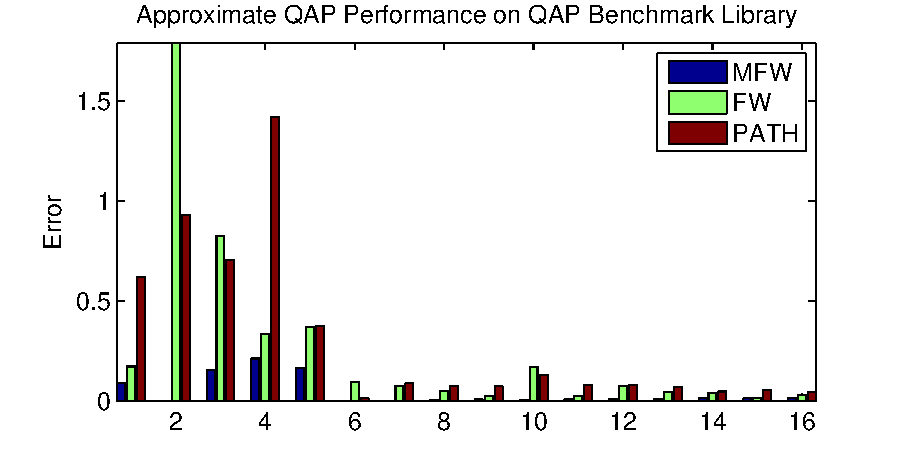
\includegraphics[width=1.0\linewidth]{../figs/benchmarks.pdf}
	\caption{relative performance plot. XXX: would a log yscale be better?}
	\label{fig:fwpath}
\end{figure}


\subsection{Simulations}

For each of the 3 below simulations, $V=10$, $n=1000$.  The results consistent show that multiple iterations of 1-QAP improve the objective function, but do not improve the misclassification rate.  This led us to investigate the relationship between QAP and Linear Assignment Problem (LAP).


\begin{figure}[ht]
\centering
\subfigure[model]{
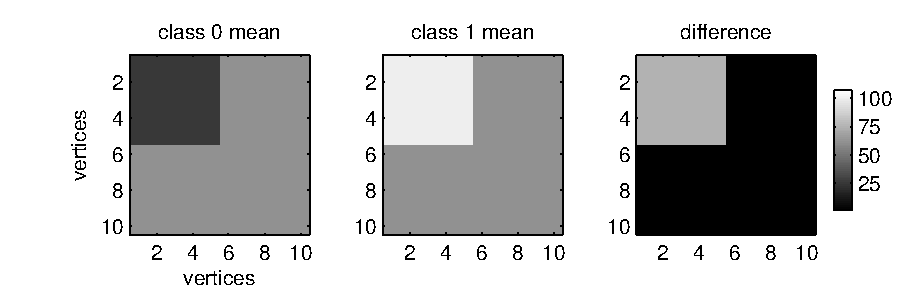
\includegraphics[scale=0.5]{../figs/homo_kidney_egg_model}
\label{fig:subfig1}
}
\subfigure[objective function]{
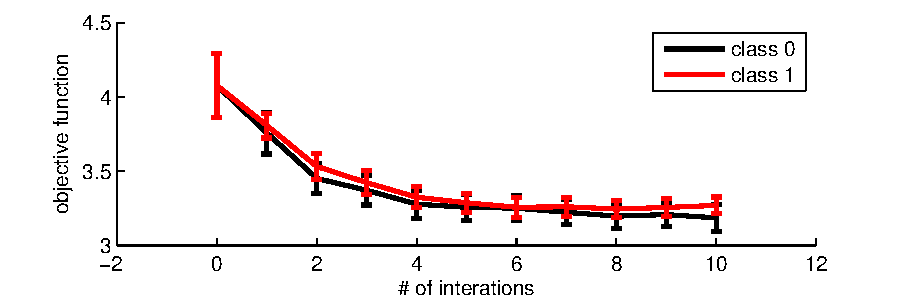
\includegraphics[scale=0.5]{../figs/homo_kidney_egg_obj}
\label{fig:subfig2}
}
\subfigure[Lhat +/- Lstd]{
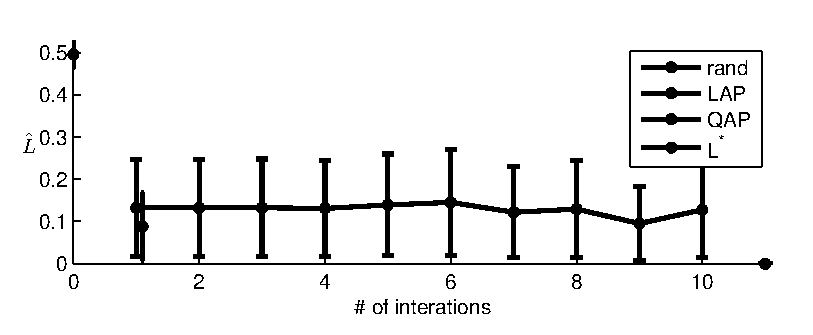
\includegraphics[scale=1]{../figs/homo_kidney_egg_Lhats}
\label{fig:subfig3}
}
\label{fig:subfigureExample}
\caption{homo kidney egg model}
\end{figure}



\begin{figure}[ht]
\centering
\subfigure[model]{
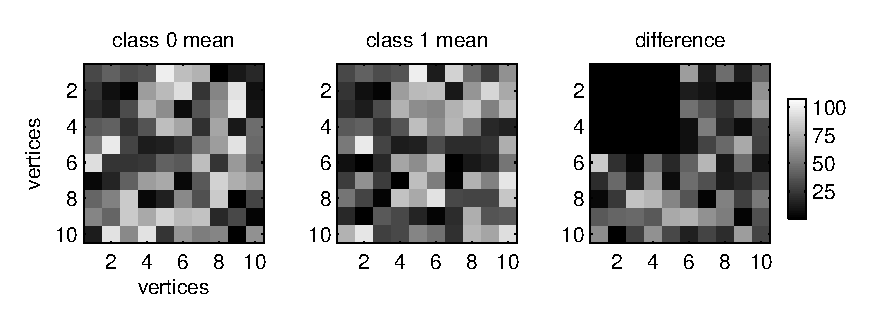
\includegraphics[scale=0.5]{../figs/hetero_kidney_egg_model}
\label{fig:subfig1}
}
\subfigure[objective function]{
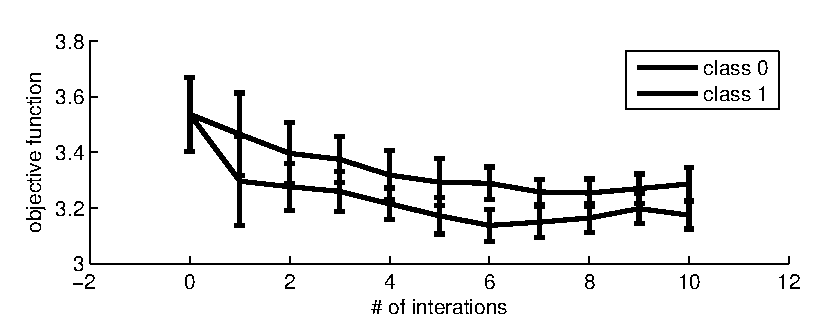
\includegraphics[scale=0.5]{../figs/hetero_kidney_egg_obj}
\label{fig:subfig2}
}
\subfigure[Lhat +/- Lstd]{
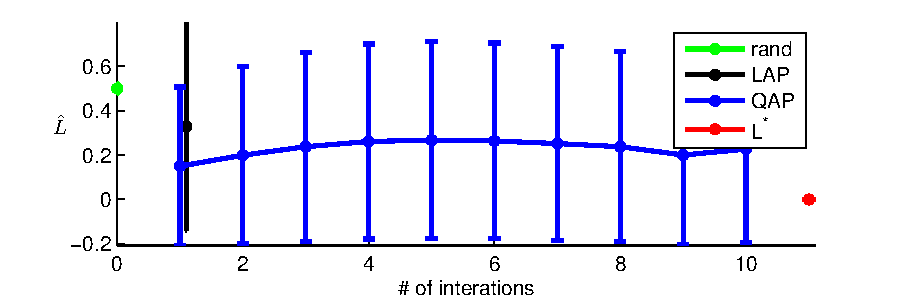
\includegraphics[scale=1]{../figs/hetero_kidney_egg_Lhats}
\label{fig:subfig3}
}
\label{fig:subfigureExample}
\caption{hetero kidney egg model}
\end{figure}



\begin{figure}[ht]
\centering
\subfigure[model]{
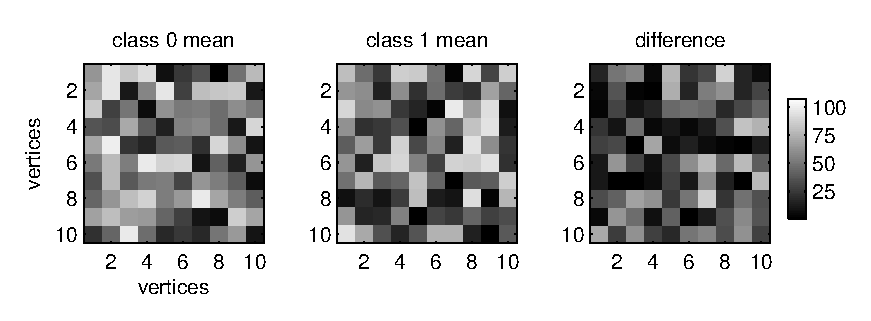
\includegraphics[scale=0.5]{../figs/hetero_model}
\label{fig:subfig1}
}
\subfigure[objective function]{
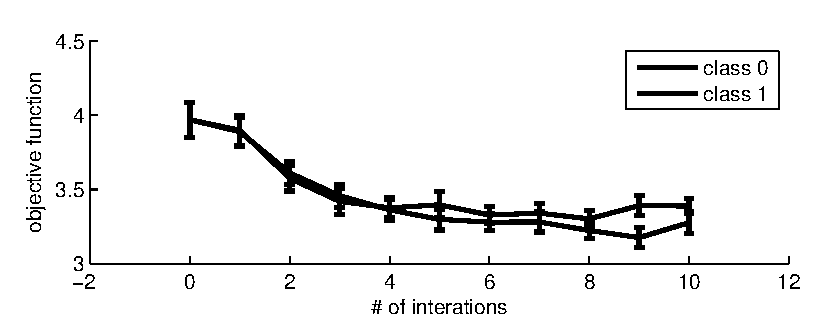
\includegraphics[scale=0.5]{../figs/hetero_obj}
\label{fig:subfig2}
}
\subfigure[Lhat +/- Lstd]{
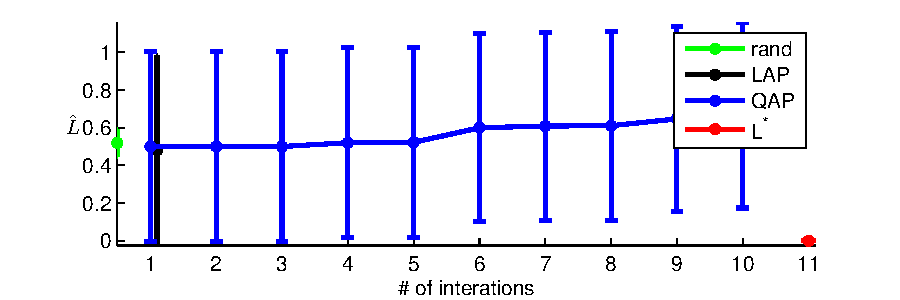
\includegraphics[scale=1]{../figs/hetero_Lhats}
\label{fig:subfig3}
}
\label{fig:subfigureExample}
\caption{hetero model}
\end{figure}





\clearpage

\subsection{LAP vs. QAP} % (fold)
\label{sub:lap_vs_qap}

LAPs can be cast as follows:

The LAP approximation  for this class problem is given by the following equation:
\begin{align} \label{eq:LAP}
	\mh{Q}_{\text{LAP}} = \argmin_{Q \in \mc{Q}} \norm{A Q\T - B }^2_F,
\end{align}
which is quite similar to QAP, except $A$ is only post-multiplied by $Q$, instead of also being pre-multiplied by $Q$. To solve a LAP, we compute the gradient of $f'(Q)=\norm{AQ\T-B}_F^2$:
\begin{align} \label{eq:grad2}
	\nabla_{Q'}^{(k)} = 2A B\T. 
\end{align}
Interestingly, this is identical to the gradient of QAP, Eq. \eqref{eq:grad}, when $Q^{(k)}$ is the identical matrix.  Thus, if QAP is initialized at the identity matrix, the first iteration is identical to LAP.  This suggests that for certain problems, LAP is both an efficient and useful approximation to graph matching.  We confirm this intuition by replacing QAP with LAP in the above simulations.  As depicted in the above figures, this intuition is consistent with the numerical results. In other words, while naively one might implement an algorithm with exponential time complexity, LAP, which is only quadratic complexity, will often suffice.


% subsection lap_vs_qap (end)

\subsection{Connectome Classification} % (fold)
\label{sub:connectome_classification}

A ``connectome'' is a graph in which vertices correspond to biological neural units, and edges correspond to connections between the units.  Diffusion Magnetic Resonance (MR) Imaging and related technologies are making the acquisition of MR connectomes routine [cite].  We use 49 subjects from the Baltimore Longitudinal Study on Aging, with acquisition and connectome inference details as reported in [cite].  For each connectome, we obtain a $70 \times 70$ element adjacency matrix, where each element of the matrix encodes the number of streamlines between a pair of regions [FACT cite], ranging between 0 and about 65,000.  Associated with each graph is class label based on the gender of the individual (24 males, 25 females).  Because the vertices are labeled, we can compare the results of having the labels and not having the labels.  As such, we implement the following classification strategies.  In each case, we use a leave-one-out strategy:

\begin{enumerate}
	\item Using the vertex labels, implement a standard $1$nn classifier, where distance is the norm of the difference between any pair of adjacency matrices.
	\item Permute only the vertex labels of the test graph, and then implement $1$nn$\circ$1-QAP.
	\item Permuting the vertex labels, then implement $1$nn$\circ$1-QAP as described above.
	\item Permuting the vertex labels, QAP each of the 48 training graphs to the test graph.  Then, given those permuted adjacency matrices, compute the average, and then implement a standard $1$nn classifier.
	\item Use the graph invariant approach as described above. We provide the normalized graph invariants as inputs into a number of standard classifiers, including $k$nn, linear classifiers, support vector machines, random forests, and CW. On this data, the CW classifier performed best; we therefore only report its results.
\end{enumerate}


\begin{table}[h!]
\caption{MR Connectome Classification Results}
\begin{center}
\begin{tabular}{|r|r|r|r|r|}
\hline
1 & 2  & 3 & 4 & 5\\
\hline
$20\%$ & $31\%$ & $45\%$ & ?? & $25\%$ \\
    \hline
\end{tabular}
\end{center}
\label{tab:fwpath}
\end{table}%



% subsection connectome_classification (end)
% 
% \paragraph{model 1: symmetric model in which LAP=1 iter of QAP} % (fold)
% \label{par:homogeneous_kidney_egg_simulation}
% 
% fig 1: model params
% 
% proof that LAP=QAP.
% 
% fig 2: numerical confirmation of proof: Lhat vs. \# iters of FW
% 
% possible simulation details: Homogeneous kidney-egg simulation: For the homogeneous kidney-egg simulations, we assume $n=10$, so $\eta^y \in (0,1)^{n\times n}$.  We further assume a stochastic block model, with two blocks, for both classes.  For class 0, $\eta_{ij}^0=q_0=0.25$ for $i,j \in [3]$, and for class 1, $\eta_{ij}^1=q_1=0.75$ for $i,j \in [3]$.  In both classes, $\eta_{ij}=p=0.5$ for $i,j \in \{4,\ldots 10\}$.  See Figure \ref{fig:models} (top row) for a graphical depiction of this model.  
% 
% 
% 
% 
% % paragraph homogeneous_kidney_egg_simulation (end)
% 
% \paragraph{perhaps: model 2: assymetric model in which LAP $<$ QAP (fig 2: show model params)} % (fold)
% \label{par:homogeneous_kidney_egg_simulation}
% 
% (this one we do depending on the results from the below synthetic data analysis (SDA).  if the SDA results are much different than the above results, this warrants a ``linking'' simulated result.)
% 
% perhaps: Heterogeneous simulation: For the heterogeneous simulations, we assume $n=10$, so $\eta^y \in (0,1)^{n\times n}$.  We further assume that each $\eta_{ij}^y \overset{iid}{\sim}$Uniform$(0,1)$.  See Figure \ref{fig:models} (bottom) row for a graphical depiction of this model.
% 
% same figures as above.
% 
% \paragraph{synthetic data} % (fold)
% \label{par:synthetic_data}
% 
% 49 subjects: 25 male, 24 female.  each with 70x70 symmetric binary matrix.  
% 
% figure 3: plot mean male, mean female, significant difference matrix.
% 
% labeled results: naive bayes performance around $70\%$.  finding signal subgraph performance around $85\%$.  
% 
% fig 4: unlabeled results: Lhat vs. \# iters of FW (we scrabble labels).  
% 
% NB: we might want to add a table (like the benchmark results) showing average performance of QAP for these guys
% 
% % paragraph synthetic_data (end)



\section{Discussion}


In this work, we have presented a number of approaches one could take 


\bibliography{/Users/joshyv/Research/latex/biblist}
\addcontentsline{toc}{section}{References}
%\bibliographystyle{apalike}
\bibliographystyle{ieeetr}
%\bibliographystyle{nature}


\end{document}